\hypertarget{alvin-simon-theodore}{%
\section{Alvin, Simon, Theodore}\label{alvin-simon-theodore}}

\begin{figure}[!ht]
  \begin{adjustwidth}{-\oddsidemargin-1in}{-\rightmargin}
    \centering
    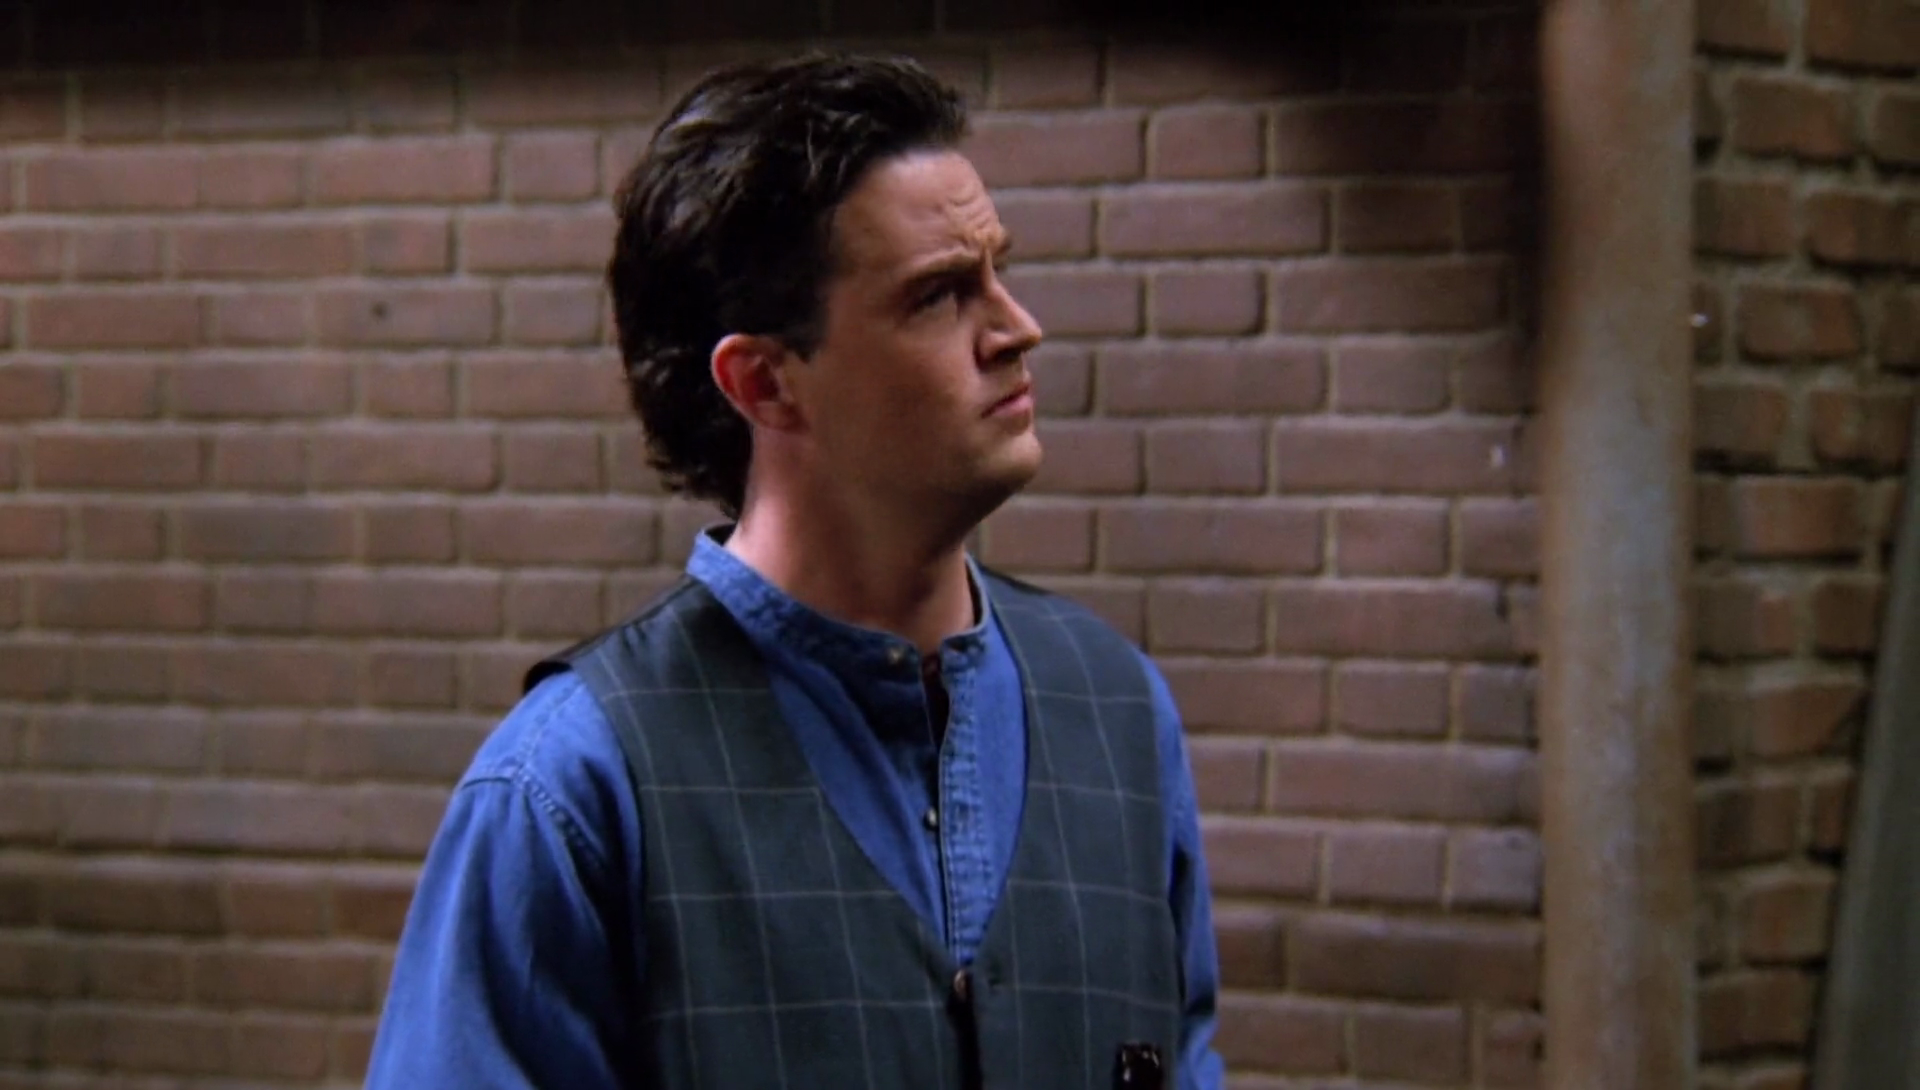
\includegraphics[trim={0 9cm 0 2cm,}, clip, width=\paperwidth]{./S01/img/24/alvin-simon-theodore.png}
    % \caption{Alvin, Simon, Theodore\label{fig:alvin-simon-theodore}}
  \end{adjustwidth}
\end{figure}

\begin{tcolorbox}[enhanced,center upper,
    drop fuzzy shadow southeast, boxrule=0.3pt,
    lower separated=false, breakable,
    colframe=black!30!dialogoBorder,colback=white]
\begin{minipage}[c]{0.16\linewidth}
  \raisebox{\dimexpr-\height+\ht\strutbox\relax}{
    \centering 
\includegraphics[width=1.4cm]{./assets/img/ross.png}
  }
   & \centering \scriptsize{Ross}
\end{minipage}
\hfill
\begin{minipage}[c]{0.8\linewidth}
  \textbf{- Do you guys know who Carl is?}\\
  - Alguém sabe quem é esse tal de Carl?
\end{minipage}

\medskip
\begin{minipage}[c]{0.16\linewidth}
  \raisebox{\dimexpr-\height+\ht\strutbox\relax}{
    \centering 
\includegraphics[width=1.4cm]{./assets/img/chandler.png}
  }
   & \centering \scriptsize{Chandler}
\end{minipage}
\hfill
\begin{minipage}[c]{0.8\linewidth}
  \textbf{- Let's see. Alvin, Simon, Theodore... No.}\\
  - Deixa eu ver. Alvin, Simon, Theodore... Não.
\end{minipage}
\end{tcolorbox}

\saveparinfos
\noindent
\begin{minipage}[c]{0.4\textwidth}\useparinfo

Ross descobre que Rachel saiu para beber com um tal de Carl, e quando
pergunta aos amigos se eles o conhecem, Chandler faz referência aos
personagens de \emph{Alvin \& the Chipmunks} (1983-1990), série animada
americana estrelada por esquilos. A série é um pouco mais antiga mas
começou a passar na NBC, mesma rede de TV de Friends, em 83.\footnote{\sloppy Alvin \& the Chipmunks - IMDB. \url{https://www.imdb.com/title/tt0084972/}}

\end{minipage}\hfill
\begin{minipage}[c]{0.6\textwidth}

\begin{figure}
  \centering
  \begin{tikzpicture}
    \node [inner sep=0pt] at (0,0) {
      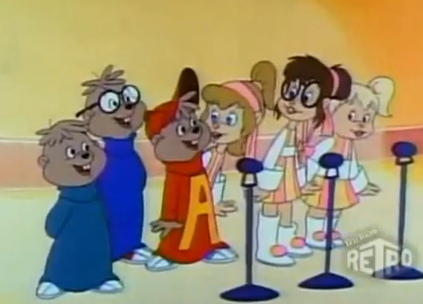
\includegraphics[width=0.8\textwidth,keepaspectratio]{./S01/img/24/alvin-chipmunks.png}
    };
    \draw [white, rounded corners=\ClipSep, line width=\ClipSep]
    (current bounding box.north west) --
    (current bounding box.north east) --
    (current bounding box.south east) --
    (current bounding box.south west) -- cycle
    ;
    \end{tikzpicture}
    \caption{Alvin & the Chipmunks\label{fig:alvin-the-chipmunks}}
\end{figure}

\end{minipage}

\hypertarget{the-three-musketeers}{%
\section{The Three Musketeers}\label{the-three-musketeers}}

\begin{figure}[!ht]
  \begin{adjustwidth}{-\oddsidemargin-1in}{-\rightmargin}
    \centering
    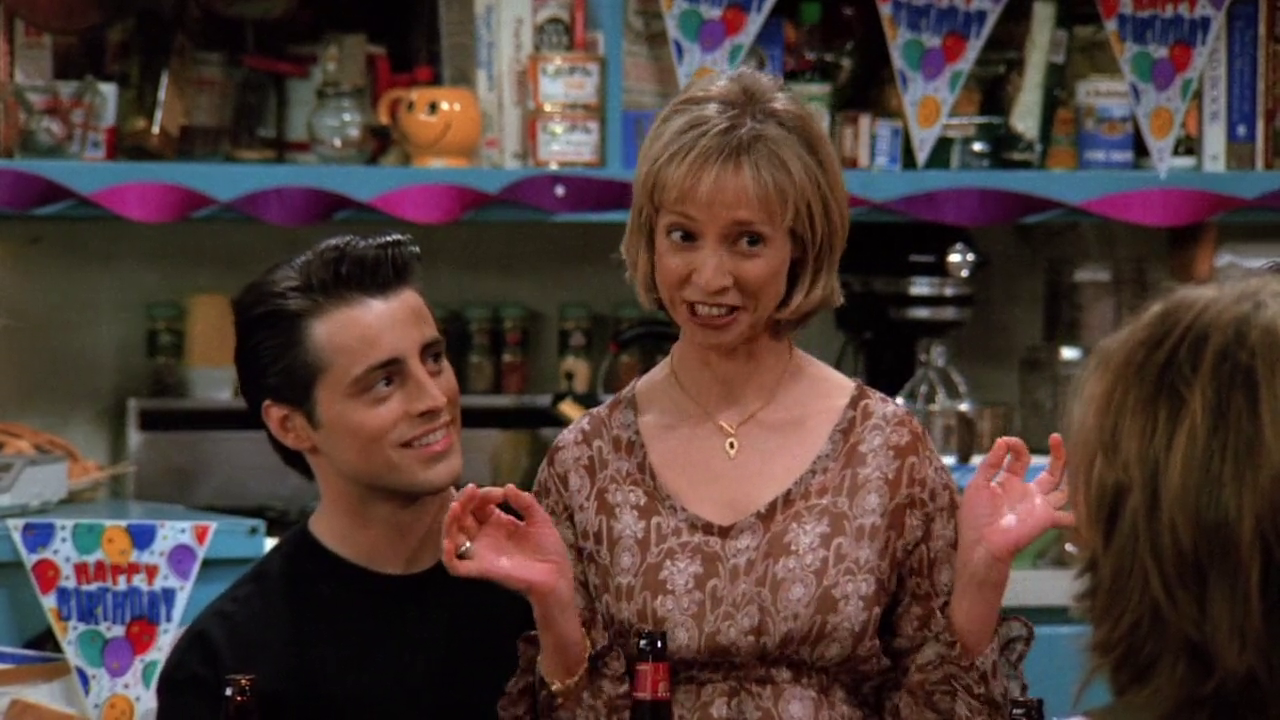
\includegraphics[trim={0 8cm 0 5cm,}, clip, width=\paperwidth]{./S01/img/24/the-three-musketeers.png}
    % \caption{The Three Musketeers\label{fig:the-three-musketeers}}
  \end{adjustwidth}
\end{figure}

\begin{tcolorbox}[enhanced,center upper,
    drop fuzzy shadow southeast, boxrule=0.3pt,
    lower separated=false, breakable,
    colframe=black!30!dialogoBorder,colback=white]
\begin{minipage}[c]{0.16\linewidth}
  \raisebox{\dimexpr-\height+\ht\strutbox\relax}{
    \centering 
\includegraphics[width=1.4cm]{./assets/img/joey.png}
  }
   & \centering \scriptsize{Joey}
\end{minipage}
\hfill
\begin{minipage}[c]{0.8\linewidth}
  \textbf{- Like "The Three Musketeers", only with fruit.}\\
  - Igual aos "Três Mosqueteiros", mas com frutas.
\end{minipage}
\end{tcolorbox}

Melanie, namorada de Joey, fala sobre como abriu o próprio negócio
vendendo cestas de frutas, e faz um trocadilho com \emph{The Three
Musketeers} (1844), um romance de \emph{Alexandre Dumas} (1802-1870)
publicado originalmente em francês, \emph{Les Trois Mousquetaires}. O
livro conta a história de um jovem chamado \emph{D'Artagnan} em busca de
fazer parte da guarda real do rei da França ao lado de \emph{Athos},
\emph{Porthos} e \emph{Aramis}.\footnote{\sloppy The Three Musketeers - Encyclopædia Britannica. \url{https://www.britannica.com/topic/The-Three-Musketeers}}

Uma versão longa-metragem foi feita em 1993 e outra em 2011.

\hypertarget{travel-scrabble}{%
\section{Travel Scrabble}\label{travel-scrabble}}

\begin{figure}[!ht]
  \begin{adjustwidth}{-\oddsidemargin-1in}{-\rightmargin}
    \centering
    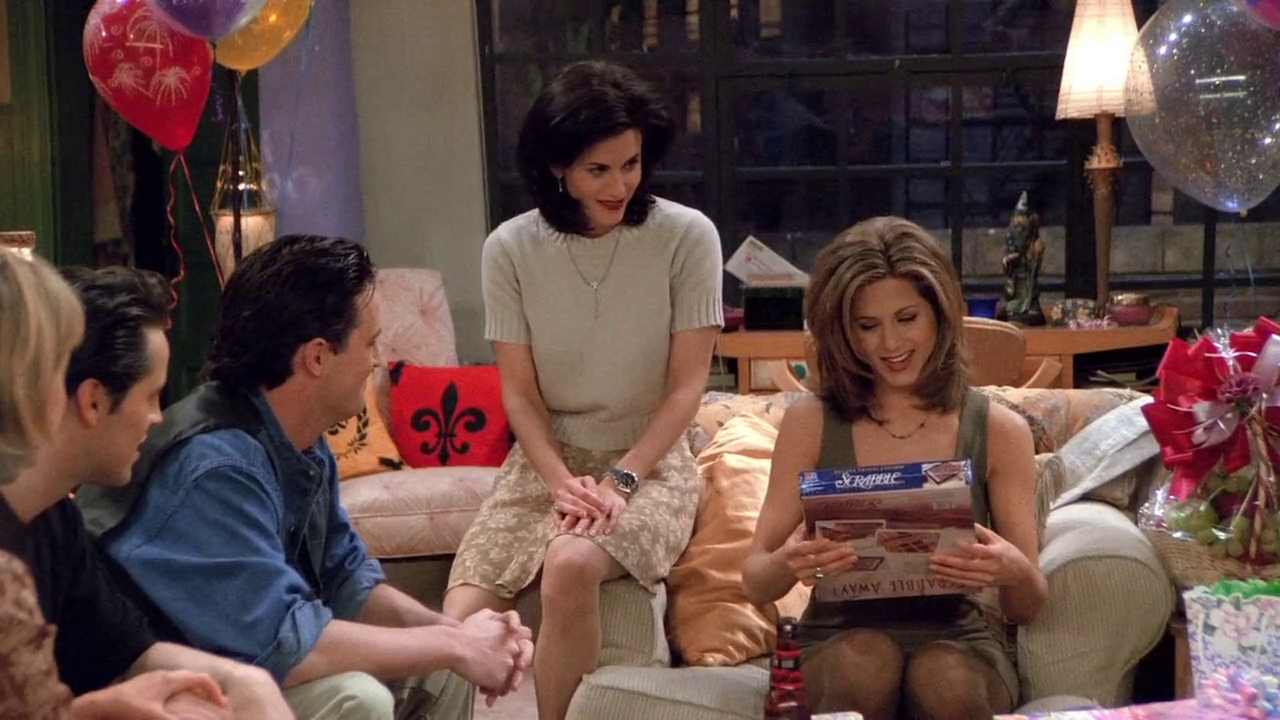
\includegraphics[trim={0 6cm 0 3cm,}, clip, width=\paperwidth]{./S01/img/24/travel-scrabble.png}
    % \caption{Travel Scrabble\label{fig:travel-scrabble}}
  \end{adjustwidth}
\end{figure}

\begin{tcolorbox}[enhanced,center upper,
    drop fuzzy shadow southeast, boxrule=0.3pt,
    lower separated=false,
    colframe=black!30!dialogoBorder,colback=white]
\begin{minipage}[c]{0.16\linewidth}
  \raisebox{\dimexpr-\height+\ht\strutbox\relax}{
    \centering 
\includegraphics[width=1.4cm]{./assets/img/rachel.png}
  }
   & \centering \scriptsize{Rachel}
\end{minipage}
\hfill
\begin{minipage}[c]{0.8\linewidth}
  \textbf{- It rattles. It's... Travel Scrabble.}\\
  - Faz barulho. É... Palavras Cruzadas para viagem.
\end{minipage}
\end{tcolorbox}

Versão de viagem do jogo \emph{Scrabble}, já citado em
\textbf{\textcolor{primarycolor}{S01E17 - Aquele com Duas Partes (Parte 2)}},
onde as peças fixam-se no tabuleiro.

\hypertarget{dr.-seuss}{%
\section{Dr.~Seuss}\label{dr.-seuss}}

\begin{figure}[!ht]
  \begin{adjustwidth}{-\oddsidemargin-1in}{-\rightmargin}
    \centering
    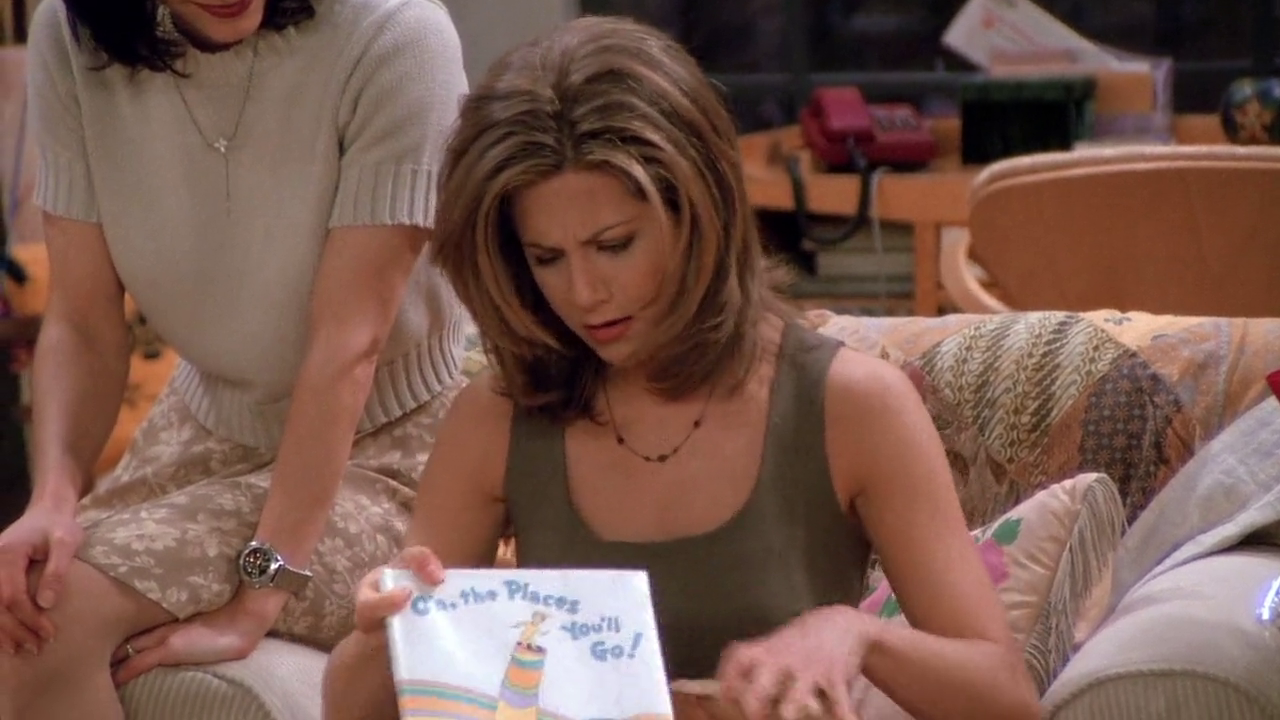
\includegraphics[trim={0 2cm 0 4cm,}, clip, width=\paperwidth]{./S01/img/24/dr-seuss.png}
    % \caption{Dr. Seuss\label{fig:dr-seuss}}
  \end{adjustwidth}
\end{figure}

\begin{tcolorbox}[enhanced,center upper,
    drop fuzzy shadow southeast, boxrule=0.3pt,
    lower separated=false, breakable,
    colframe=black!30!dialogoBorder,colback=white]
\begin{minipage}[c]{0.16\linewidth}
  \raisebox{\dimexpr-\height+\ht\strutbox\relax}{
    \centering 
\includegraphics[width=1.4cm]{./assets/img/rachel.png}
  }
   & \centering \scriptsize{Rachel}
\end{minipage}
\hfill
\begin{minipage}[c]{0.8\linewidth}
  \textbf{- Feels like a book. And it's a book!}\\
  - Parece um livro. É um livro!
\end{minipage}

\medskip
\begin{minipage}[c]{0.16\linewidth}
  \raisebox{\dimexpr-\height+\ht\strutbox\relax}{
    \centering 
\includegraphics[width=1.4cm]{./assets/img/phoebe.png}
  }
   & \centering \scriptsize{Phoebe}
\end{minipage}
\hfill
\begin{minipage}[c]{0.8\linewidth}
  \textbf{- It's Dr. Seuss!}\\
  - É Dr. Seuss!
\end{minipage}
\end{tcolorbox}

\saveparinfos
\noindent
\begin{minipage}[c]{0.5\textwidth}\useparinfo

Rachel ganha o livro \emph{Oh, the Places You'll Go!} (1990) de Joey.
Foi o último livro publicado de \emph{Dr.~Seuss} (já citado no episódio
\textbf{\textcolor{primarycolor}{S01E09 - Aquele em que o Underdog Escapa}})
e fala sobre a jornada da vida e seus desafios.\footnote{\sloppy Oh, the Places You’ll Go! - Dr. Seuss - Google Books. \url{https://books.google.com.br/books/about/Oh_the_Places_You_ll_Go.html?id=_LettPDhwR0C\&redir_esc=y}}

\end{minipage}\hfill
\begin{minipage}[c]{0.5\textwidth}

\begin{figure}
  \centering
  \begin{tikzpicture}
    \node [inner sep=0pt] at (0,0) {
      
\includegraphics[width=0.7\textwidth,keepaspectratio]{./S01/img/24/places-book.jpg}
    };
    \draw [white, rounded corners=\ClipSep, line width=\ClipSep]
    (current bounding box.north west) --
    (current bounding box.north east) --
    (current bounding box.south east) --
    (current bounding box.south west) -- cycle
    ;
    \end{tikzpicture}
    \caption{Oh, the Places You’ll Go!\label{fig:oh-the-places-you-ll-go}}
\end{figure}

\end{minipage}

Joey menciona que o livro o ajudou em momentos difíceis, mas na época de
lançamento ele teria uns 20 anos.

\hypertarget{hitchcock-and-scarface}{%
\section{Hitchcock and Scarface}\label{hitchcock-and-scarface}}

\begin{figure}[!ht]
  \begin{adjustwidth}{-\oddsidemargin-1in}{-\rightmargin}
    \centering
    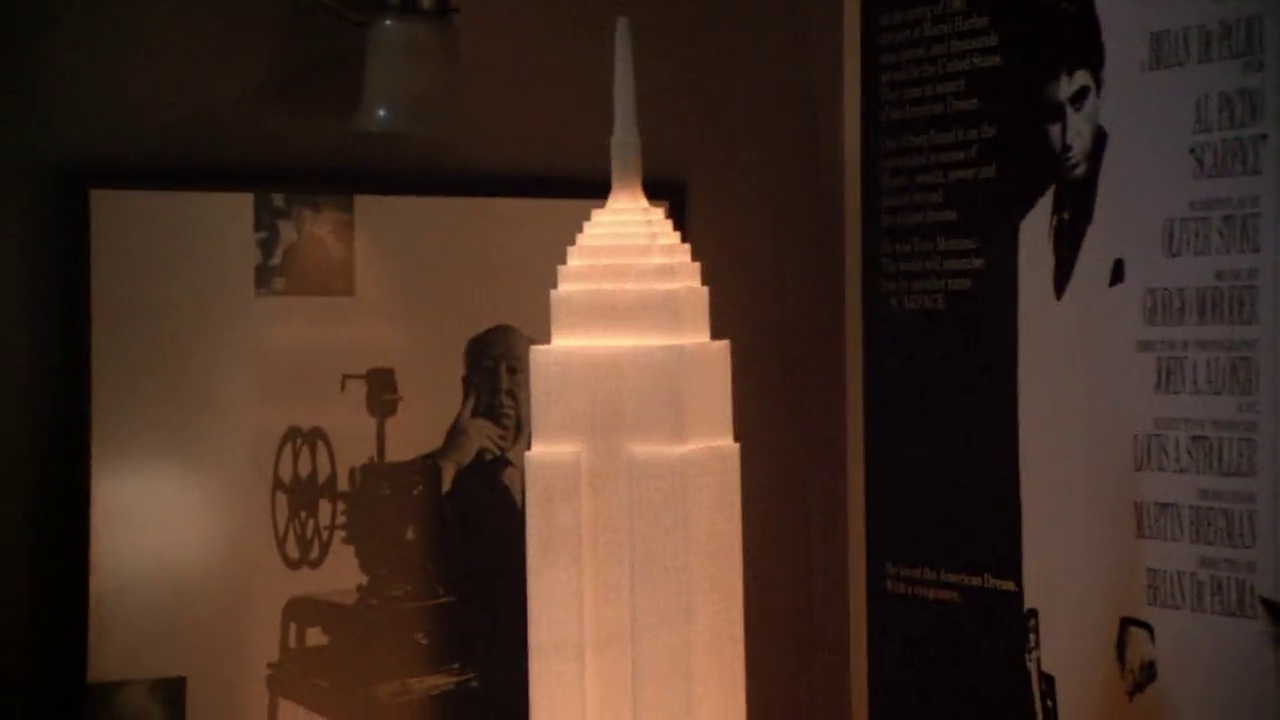
\includegraphics[trim={0 7cm 0 2cm,}, clip, width=\paperwidth]{./S01/img/24/scarface-and-hitchcock.png}
    % \caption{Scarface and Hitchcock\label{fig:scarface-and-hitchcock}}
  \end{adjustwidth}
\end{figure}

No quarto de Joey é possível ver pôsteres de \emph{Alfred Hitchcock}
(1899-1980) (à esquerda), diretor Inglês famoso por filmes de suspense,
entre eles \emph{Psycho} (1960), \emph{Psicose} no Brasil\footnote{\sloppy Alfred Hitchcock - Encyclopædia Britannica. \url{https://www.britannica.com/biography/Alfred-Hitchcock}};
e um pôster do filme \emph{Scarface} (1983) (à direita), filme estrelado
por \emph{Al Pacino}, ator já citado no episódio
\textbf{\textcolor{primarycolor}{S01E06 - Aquele com o Traseiro}}. Nele
o personagem de \emph{Al}, \emph{Tony Montana}, um criminoso cubano, é
deportado para \emph{Miami} e toma controle de um grande cartel de
drogas.\footnote{\sloppy Scarface - IMDB. \url{https://www.imdb.com/title/tt0086250/}}

\hypertarget{hey-big-spender}{%
\section{Hey big\ldots{} spender}\label{hey-big-spender}}

\begin{figure}[!ht]
  \begin{adjustwidth}{-\oddsidemargin-1in}{-\rightmargin}
    \centering
    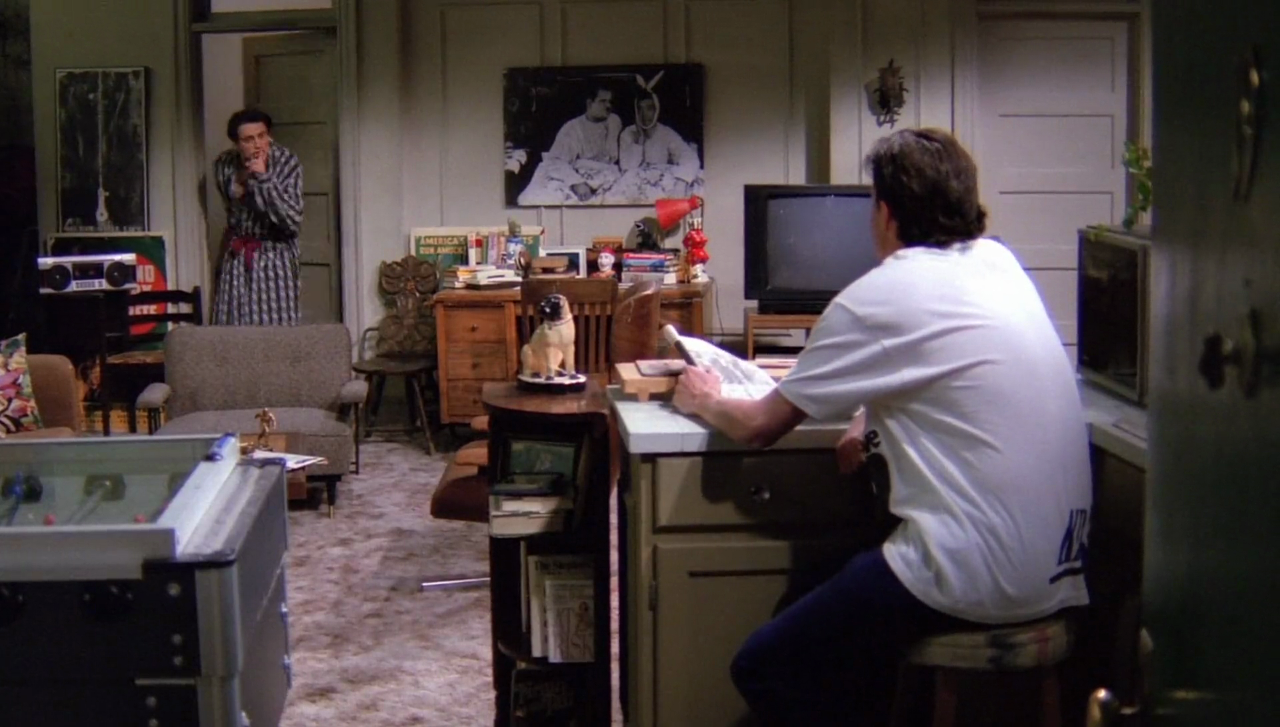
\includegraphics[trim={0 10cm 0 3cm,}, clip, width=\paperwidth]{./S01/img/24/hey-big-spender.png}
    % \caption{Hey big… spender\label{fig:hey-big-spender}}
  \end{adjustwidth}
\end{figure}

\begin{tcolorbox}[enhanced,center upper,
    drop fuzzy shadow southeast, boxrule=0.3pt,
    lower separated=false, breakable,
    colframe=black!30!dialogoBorder,colback=white]
\begin{minipage}[c]{0.16\linewidth}
  \raisebox{\dimexpr-\height+\ht\strutbox\relax}{
    \centering 
\includegraphics[width=1.4cm]{./assets/img/chandler.png}
  }
   & \centering \scriptsize{Chandler}
\end{minipage}
\hfill
\begin{minipage}[c]{0.8\linewidth}
  \textbf{- Hey, big...}\\
  - Ei, grande...
\end{minipage}

\medskip
\begin{minipage}[c]{0.16\linewidth}
  \raisebox{\dimexpr-\height+\ht\strutbox\relax}{
    \centering 
\includegraphics[width=1.4cm]{./assets/img/joey.png}
  }
   & \centering \scriptsize{Joey}
\end{minipage}
\hfill
\begin{minipage}[c]{0.8\linewidth}
  \textbf{- Shh!}\\
  - Shh!
\end{minipage}

\medskip
\begin{minipage}[c]{0.16\linewidth}
  \raisebox{\dimexpr-\height+\ht\strutbox\relax}{
    \centering 
\includegraphics[width=1.4cm]{./assets/img/chandler.png}
  }
   & \centering \scriptsize{Chandler}
\end{minipage}
\hfill
\begin{minipage}[c]{0.8\linewidth}
  \textbf{- Spender.}\\
  - Gastador.
\end{minipage}
\end{tcolorbox}

Joey levanta-se antes de Melanie e Chandler faz uma referência ao
musical \emph{Sweet Charity} (1966) --- que também virou filme em 1969
---, que conta a história de uma dançarina de cabaré que não perde a
esperança de encontrar um grande amor. A canção \emph{Big Spender} é um
dos pontos altos do musical.\footnote{\sloppy Sweet Charity - IBDB. \url{https://www.ibdb.com/broadway-production/sweet-charity-3281}}

\bigskip
\begin{tcolorbox}[enhanced,
    drop fuzzy shadow southeast, boxrule=0.3pt,
    lower separated=false, sidebyside, sidebyside align=top,
    halign=flush right, halign lower=left, breakable,
    colframe=black!30!dialogoBorder,colback=musicaBg]
\includegraphics[width=0.4cm]{./assets/img/icon-music.png}\\
Hey, big spender!\\Spend…a little time with …me!\\
\tcblower
\includegraphics[width=0.4cm]{./assets/img/icon-language.png}\\
Ei, grande gastador!\\Gaste… um pouco de tempo… comigo!\\
\end{tcolorbox}

\hypertarget{crunch-berries}{%
\section{Crunch Berries}\label{crunch-berries}}

\begin{figure}[!ht]
  \begin{adjustwidth}{-\oddsidemargin-1in}{-\rightmargin}
    \centering
    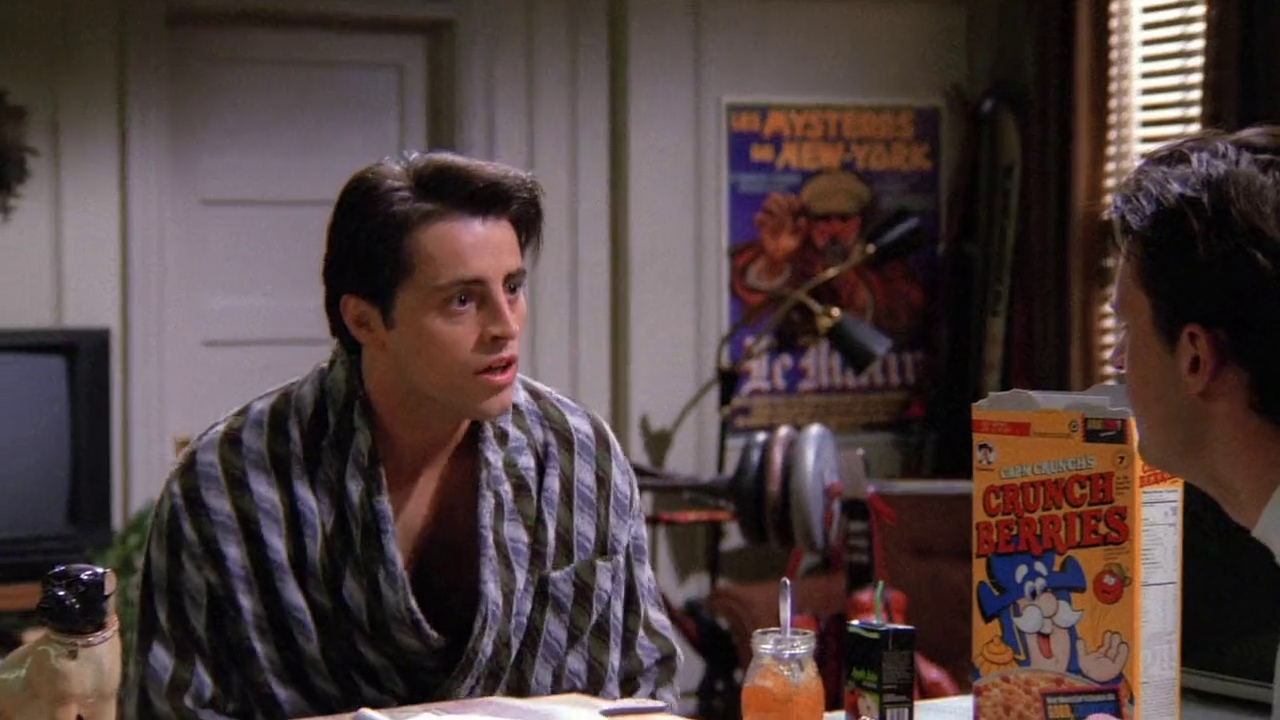
\includegraphics[trim={0 1cm 0 5cm,}, clip, width=\paperwidth]{./S01/img/24/crunch-berries.png}
    % \caption{Crunch Berries\label{fig:crunch-berries}}
  \end{adjustwidth}
\end{figure}

Conversando com Joey sobre como foi a noite com Melanie, Chandler é
visto comendo o cereal \emph{Cap'n Crunch - Crunch Berries} (1967), um
dos cereais matinais mais populares na época.\footnote{\sloppy The untold truth of Cap’n Crunch - Mashed (Inglês). \url{https://www.mashed.com/206601/the-untold-truth-of-capn-crunch/}}

\hypertarget{ed-begley-jr.}{%
\section{Ed Begley Jr.}\label{ed-begley-jr.}}

\begin{figure}[!ht]
  \begin{adjustwidth}{-\oddsidemargin-1in}{-\rightmargin}
    \centering
    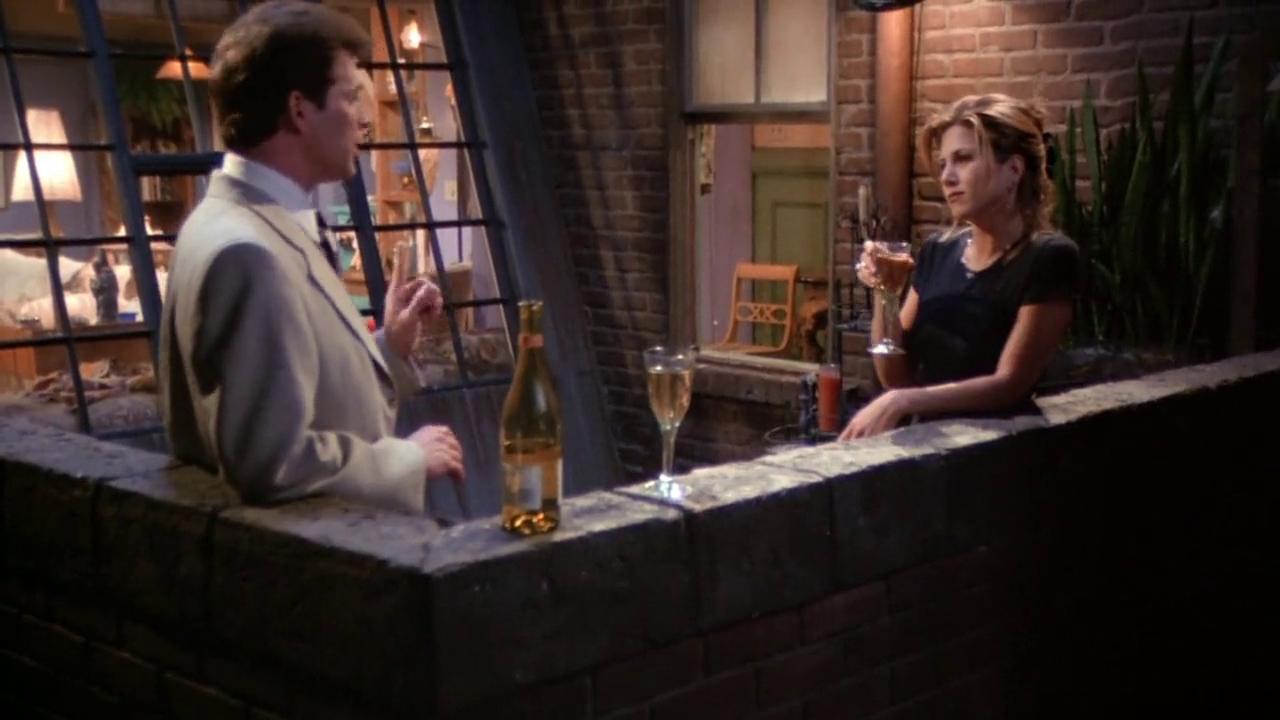
\includegraphics[trim={0 9cm 0 0cm,}, clip, width=\paperwidth]{./S01/img/24/ed-begley-jr.png}
    % \caption{Ed Begley Jr.\label{fig:ed-begley-jr}}
  \end{adjustwidth}
\end{figure}

\begin{tcolorbox}[enhanced,center upper,
    drop fuzzy shadow southeast, boxrule=0.3pt,
    lower separated=false, breakable,
    colframe=black!30!dialogoBorder,colback=white]
\begin{minipage}[c]{0.16\linewidth}
  \raisebox{\dimexpr-\height+\ht\strutbox\relax}{
    \centering 
\includegraphics[width=1.4cm]{./assets/img/carl.png}
  }
   & \centering \scriptsize{Carl}
\end{minipage}
\hfill
\begin{minipage}[c]{0.8\linewidth}
  \textbf{- If I see one more picture of Ed Begley Jr. in that stupid electric car...}\\
  - Se eu vir mais uma foto de Ed Begley Jr. naquele estúpido carro elétrico...
\end{minipage}
\end{tcolorbox}

Rachel volta ao apartamento de seu encontro com Carl, e ele menciona
\emph{Ed Begley Jr.} (1949-), ator americano e ativista do meio
ambiente. Em 1970 \emph{Ed} comprou seu primeiro carro elétrico, um
\emph{Taylor-Dunn}, que na verdade estava mais para um carrinho de golfe
com um para-brisa e uma buzina. Ele foi pioneiro no uso de carros
elétricos e financiou vários projetos.\footnote{\sloppy Actor Ed Begley electric car pioneer - Wheels.ca (Inglês). \url{https://www.wheels.ca/news/actor-ed-begley-electric-car-pioneer/}}
